\documentclass[xcolor={dvipsnames},pdf, hyperref={colorlinks=true, citecolor=ForestGreen, linkcolor=BlueViolet, urlcolor=Magenta}]{beamer}
\usetheme{Frankfurt}  
\usecolortheme{whale}
\usepackage{tikz} 
\usepackage{amsmath}
\usepackage{amsthm}
\usepackage{amssymb}              % used for \eqref{} in this document
\usepackage{dsfont}
\usepackage{hyperref}
\usepackage{threeparttable}
\usepackage{multirow}
\graphicspath{{Figures/}}
\usepackage{booktabs}
\usepackage{tikz}
\newtheorem{exmp}{Example}[section]
\usepackage{subcaption}
\usepackage{adjustbox}
\usepackage{graphicx}
\usepackage[mathscr]{euscript}
\usepackage{remreset}% tiny package containing just the \@removefromreset command
\makeatletter
\@removefromreset{subsection}{section}
\makeatother
\setcounter{subsection}{1}
\usepackage{float}
\usepackage{sgamevar}
\usepackage{sgame}

\newcommand{\defn}[1]{\textbf{#1}}


%Instructor version
\newcommand{\blank}[0]{}
\newcommand{\ddp}[1]{{\textcolor{ForestGreen}{#1}}} 
\newcommand{\dd}[1]{{\underline{\textcolor{ForestGreen}{#1}}}}

%Student version
%\newcommand{\blank}[0]{\vspace{2em}}
%\newcommand{\dd}[1]{\underline{\hspace{3cm}}} 
%\newcommand{\ddp}[1]{}

\addtobeamertemplate{navigation symbols}{}{%
	\usebeamerfont{footline}%
	\usebeamercolor[fg]{footline}%
	\hspace{1em}%
	\insertframenumber/\inserttotalframenumber
}

\section{Introduction}

%% preamble
\title{The Costs of Production}
\author{David A. D\'iaz}
\institute{UNC Chapel Hill}
\date{}

\AtBeginSection[] %Section links on slides

\begin{document} 
	
	\begin{frame}
		
		\titlepage
		
	\end{frame}
	

\begin{frame}{Industrial Organization}

\begin{itemize}
	\item \defn{Industrial Organization:} The study of how firms' decisions about prices and quantities depend on the market conditions they face.
	\item We assume that the goal of a firm is to maximize \dd{profit}. Firms earn revenue from the sale of their output: $TR = PQ$ 
	\item Moreover, firms also incurs some costs to produce. The market value of the inputs a firm uses in production are the firm's \dd{total costs}.
	\item Profit ($\Pi$) is given by \dd{$\Pi = TR - TC$}.
\end{itemize}

\end{frame}

\begin{frame}{Opportunity Costs}
\begin{itemize}
	\item 	When we talk about a firm's costs of production, we will include \textit{all} the opportunity costs of making its output. 
	\item The firm's opportunity costs are divided into two pieces:
	\begin{enumerate}
		\itemsep1em 
		\item Explicit costs: Input costs that require an outlay of money by the firm.
		\item Implicit costs: Input costs that do not require an outlay of money.
	\end{enumerate}
\end{itemize}
\end{frame}

\begin{frame}{Economic vs Accounting Profit}
\begin{itemize}
	\item 	Why do we include implicit costs? \ddp{They affect firm decisions -- opportunity costs should be taken into account.}
	\item \defn{Economic profit:} \ddp{$TR$ - (explicit costs + implicit costs). \\}
	\item \defn{Accounting profit:} \ddp{$TR$ - explicit costs.\\}
	\item Since economic profit includes implicit costs, it will generally be \dd{lower} than accounting profit.
\end{itemize}
\end{frame}

\section{Production Functions}

\begin{frame}{Production Functions}
\begin{itemize}
	\item \defn{Production Function:} Relationship between quantity of inputs used to make a good and the quantity of output.
	\blank \blank \blank \blank \blank
	\begin{figure}[H]
		\centering
		\ddp{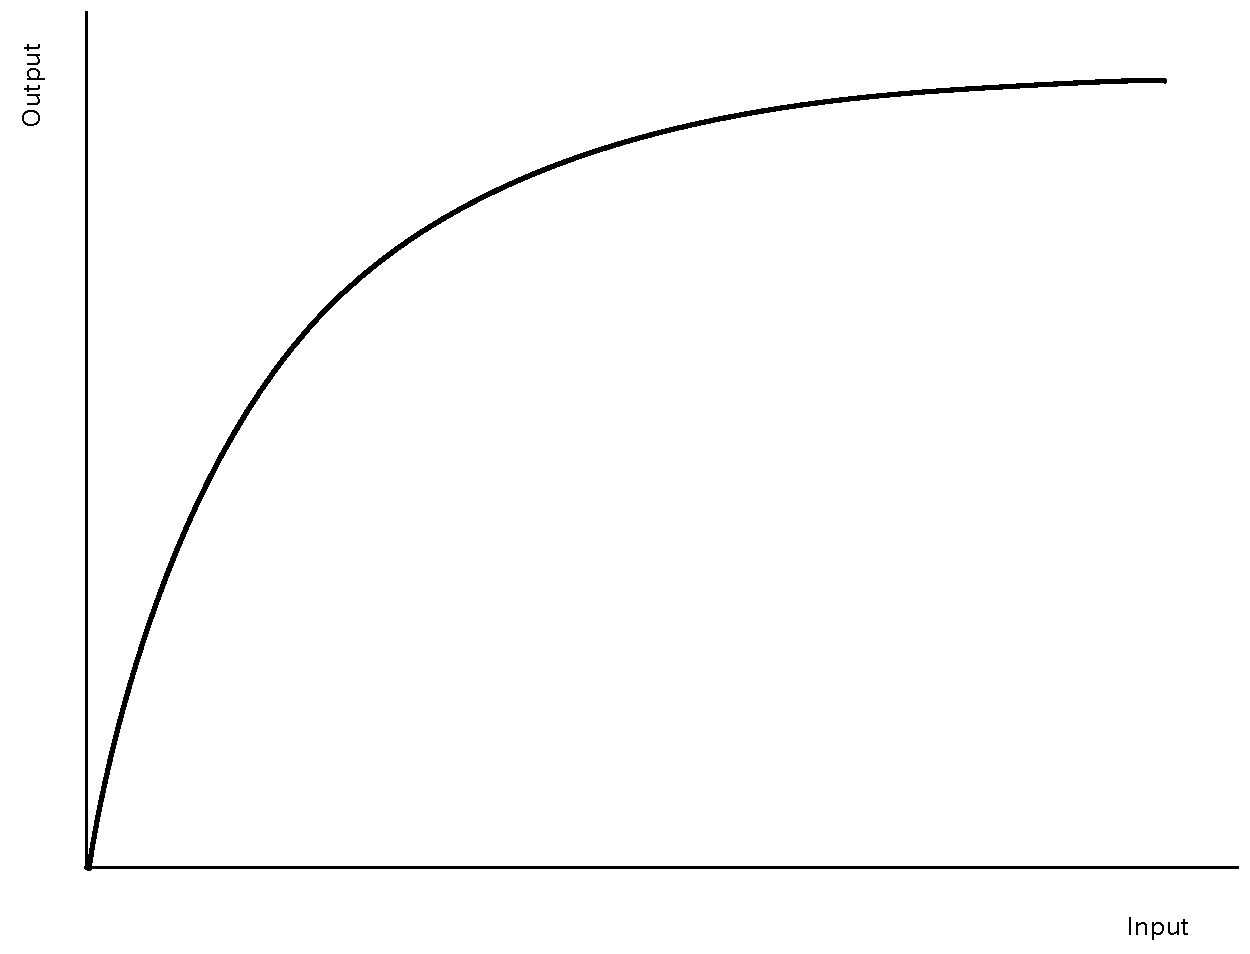
\includegraphics[scale=.30]{plot54.pdf}}
		\caption{Simplified Production Function}
	\end{figure}

\end{itemize}
\end{frame}

\begin{frame}{Production Functions}
\begin{itemize}
	\item Rational people (and firms) think \dd{on the margin}. 
	\item With this in mind, the \defn{marginal product} of an input is the \dd{increase} in \dd{output} from an additional unit of input. 
	\item Notable marginal products:
	\begin{itemize}
		\item 	$MP_L$ = \ddp{$\frac{\Delta Q}{\Delta L}$} 
		\item  	$MP_K$ = \ddp{$\frac{\Delta Q}{\Delta K}$} 
	\end{itemize}


\end{itemize}
\end{frame}

\begin{frame}{Production Functions}
	\begin{exmp}
		
		Consider Table \ref{bluth} below. What is the marginal product of labor of the second worker? The fifth? Draw a graph and show the $MP_L$ at each unit of labor.
		
		\begin{table}[ht]
			\centering
			\caption{Production of Frozen Bananas}
			\label{bluth}
			\begin{tabular}{ c|c|c}        
				
				Number of workers & Output (per day) & MPL \\
				\hline
				0 & 0 & \ddp{---} \\
				1 & 20 & \ddp{20} \\
				2 & 35 & \ddp{15} \\
				3 & 45 & \ddp{10} \\
				4 & 50 & \ddp{5} \\
				5 & 52 & \ddp{2} \\
				6 & 53 & \ddp{1} \\
			\end{tabular}
		\end{table} 
	\end{exmp}
\end{frame}

\begin{frame}[b]{Production Functions}
	\begin{figure}[H]
		\centering
		\ddp{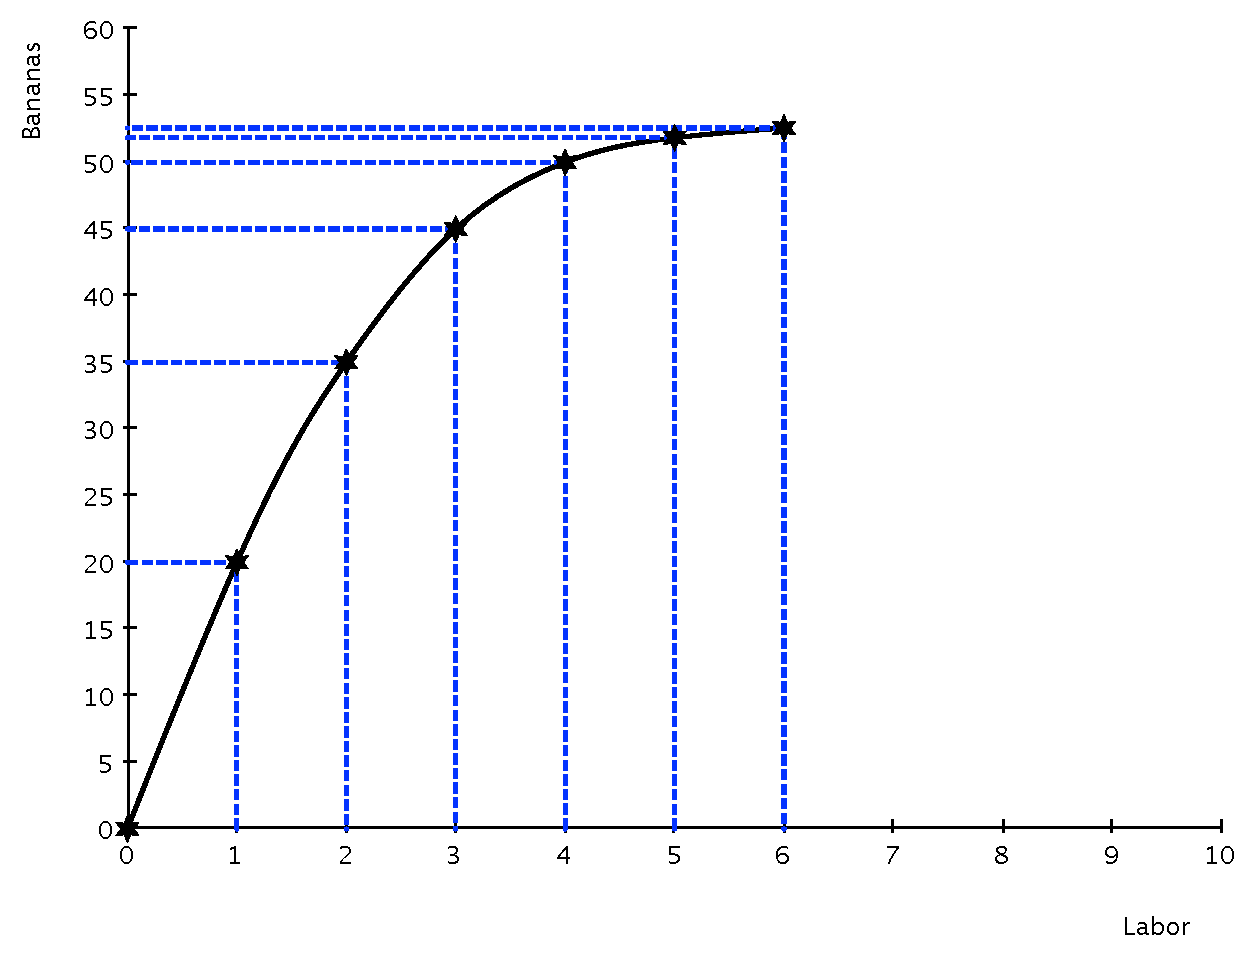
\includegraphics[scale=.40]{plot55.pdf}}
		\caption{Marginal Product of Labor}
	\end{figure}
\end{frame}


\begin{frame}{Production Functions}
	\begin{itemize}
		\item 	Properties of the Production Function:
		\begin{enumerate}
			\item An increase in inputs increases output.
			\begin{itemize}
				\item $MP_L > 0$, $MP_K > 0$
			\end{itemize}
			\item Diminishing marginal product: $MP$ declines (eventually) as the number of inputs increases.
		\end{enumerate}
	\end{itemize}
\end{frame}

\section{The Costs of Production}

\begin{frame}{The Costs of Production}
\begin{itemize}
	\item Because of diminishing marginal product, the cost curve becomes steeper as the quantity of output increases. 
	\begin{itemize}
	\item As $Q$ increases, producing an additional unit of output requires a lot of additional units of inputs and so is more costly.
	\end{itemize}
\end{itemize}
\blank \blank \blank \blank 
\begin{figure}[H]
	\centering
	\ddp{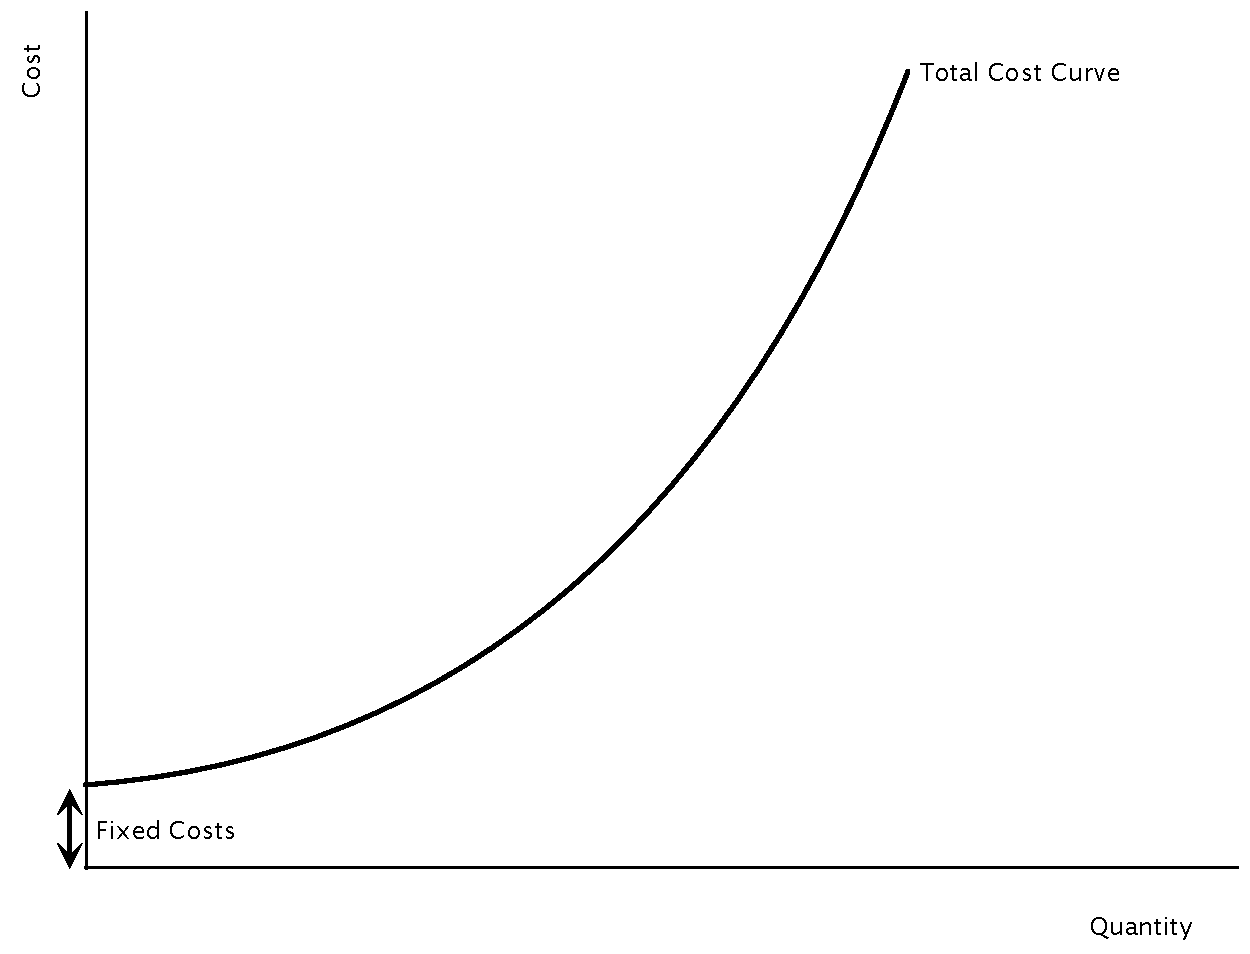
\includegraphics[scale=.3]{plot56.pdf}}
	\caption{Simplified Total Cost Curve}
\end{figure}
\end{frame}

\begin{frame}{The Costs of Production}
\begin{itemize}
	\item \defn{Fixed Costs (FC):} Costs that do not vary with the quantity of output produced.
	\item \defn{Variable Costs (VC):} Costs that vary with the quantity of output produced.
	\item If a producer does not produce any output his variable costs are \dd{zero}.
	\item \defn{Total costs (TC):} \dd{$FC + VC$}.	
\end{itemize}
\end{frame}

\begin{frame}{The Costs of Production}
\begin{itemize}
	\item \defn{Average Total Cost:} The cost of making a typical unit of output. \[ATC = TC/Q\]
	\item \defn{Average Fixed Cost:} $=FC/Q$
	\item \defn{Average Variable Cost:} $=VC/Q$
	\[ATC =\frac{FC + VC}{Q} = FC/Q + VC/Q =  AFC + AVC\]
\end{itemize}
\end{frame}

\begin{frame}{The Costs of Production}
	\begin{itemize}
		\item \defn{Marginal Cost:} The increase in total costs that arises from producing an extra unit of output.
		\[MC = \frac{\Delta TC}{\Delta Q} = \frac{\Delta VC}{\Delta Q}\]
		\item \defn{Efficient scale:} The quantity of output that minimizes $ATC$.
	\end{itemize}
\end{frame}

\begin{frame}{The Costs of Production}
	\begin{exmp} Julien also owns a juice bar, which has the following cost schedule:
		
		\begin{table}[H]
			\centering
			\caption{Production of Mango Juice}
			\begin{tabular}{ c|c|c|c|c|c}        
				
				Quantity & Variable Cost & Total Cost & AVC & ATC & MC \\
				\hline
				0 & \$0 &\$30 & \ddp{---} & \ddp{---} & \ddp{---} \\
				1 & \$10 & \$40 & \ddp{10} & \ddp{40} & \ddp{10} \\
				2 & \$25 & \$55 & \ddp{12.5} & \ddp{27.5} & \ddp{15}\\
				3 & \$45 & \$75 & \ddp{15} & \ddp{25} & \ddp{20} \\
				4 & \$70 & \$100 & \ddp{17.5} & \ddp{25} & \ddp{25} \\
				5 & \$100 & \$130 &  \ddp{20} & \ddp{26} & \ddp{30} \\
				6 & \$135 & \$165 &  \ddp{22.5} & \ddp{27.5} & \ddp{35}\\
			\end{tabular}
		\end{table} 
		
		Calculate the AVC, ATC, and MC for each quantity.
	\end{exmp}
\end{frame}

\begin{frame}{The Costs of Production}
	\begin{exmp}
		Julien's Frozen Banana stand has the following ATC schedule:
		
		\begin{table}[ht]
			\centering
			\caption{ATC of Frozen Bananas}
			\begin{tabular}{ c|c}        
				
				Quantity & Average Total Cost \\
				\hline
				600 & \$3.00 \\
				601 & \$3.01 \\
			\end{tabular}
		\end{table} 
		He made 600 bananas today and sold them all. He is about to close up shop when someone calls, desperate to escape the heat and buy a banana. She offers to pay \$5.50 for it. Should Julien accept this offer or not? Why?
	\end{exmp} 
\pause	\ddp{$MB = MR = \$5.50.$ $MC = 9.01$. Nope, don't sell since $MC>MB$.}
\end{frame}

\begin{frame}{The Costs of Production - Properties}

	\begin{enumerate}
		\item Marginal cost: Rising marginal costs (reflects diminishing $MP$). 
		\item Average fixed cost: Always decreasing since $FC$ are constant.
		\item Average variable cost: Rising due to diminishing $MP$.
		\item Average total cost: 
		\begin{itemize}
			\item U-shaped due to addition of $AFC$ \& $AVC$.
			\item At low $Q$, high $AFC$, low $AVC$ leads to high $ATC$.
			\item As $Q$ increases, $AFC$ decreases fast initially while $AVC$ increases at constant rate so $ATC$ decreases.
			\item At high $Q$, $AFC$ decreases slowly and increasing $AVC$ becomes dominant effect so $ATC$ rises.
		\end{itemize}
	\end{enumerate}
\end{frame}	

\begin{frame}[b]{The Costs of Production - Properties}
	\begin{figure}[H]
		\centering
		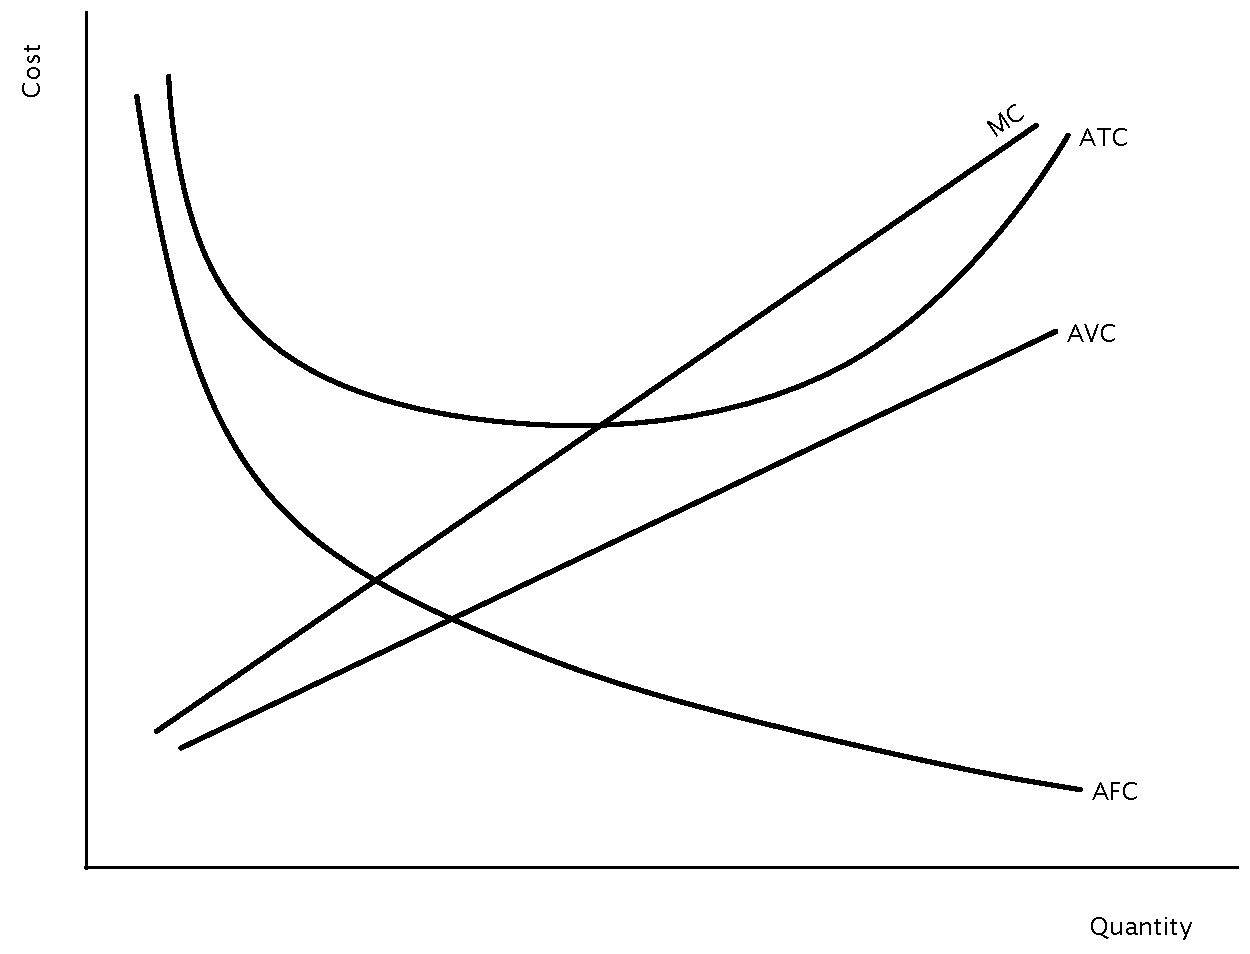
\includegraphics[scale=.35]{plot57.pdf}
		\caption{Simplified Cost Curves}
	\end{figure}
\end{frame}
	
\begin{frame}{The Costs of Production}
\begin{itemize}
	\item If we are at a level of production where marginal costs are less than average total costs, then average total costs are \dd{decreasing}.
	\item If we are at a level of production where marginal costs are greater than average total costs, then average total costs are \dd{increasing}.
\end{itemize}
\end{frame}

\begin{frame}{The Costs of Production - Properties}
	\begin{itemize}
		\item If the next unit of input adds less to production costs than current average, average cost will decrease. 
		\item If the next unit of input adds more to production costs than the current average, average cost will increase.
		\item As a result, $ATC$ and $MC$ meet at \dd{the minimum of $ATC$}.
	\end{itemize}
\end{frame}

\begin{frame}{The Costs of Production - Properties}
\begin{itemize}
	\item We made the simplifying assumption that firms exhibit decreasing marginal product for all levels of inputs in order to get the main points associated with production and costs across. 
	\item However, this is not generally the case. 
	\item Generally, $MP$ increases initially before decreasing after some level of inputs.
\end{itemize}
\end{frame}

\begin{frame}[b]{The Costs of Production - Properties}
		\begin{figure}[H]
			\centering
				\ddp{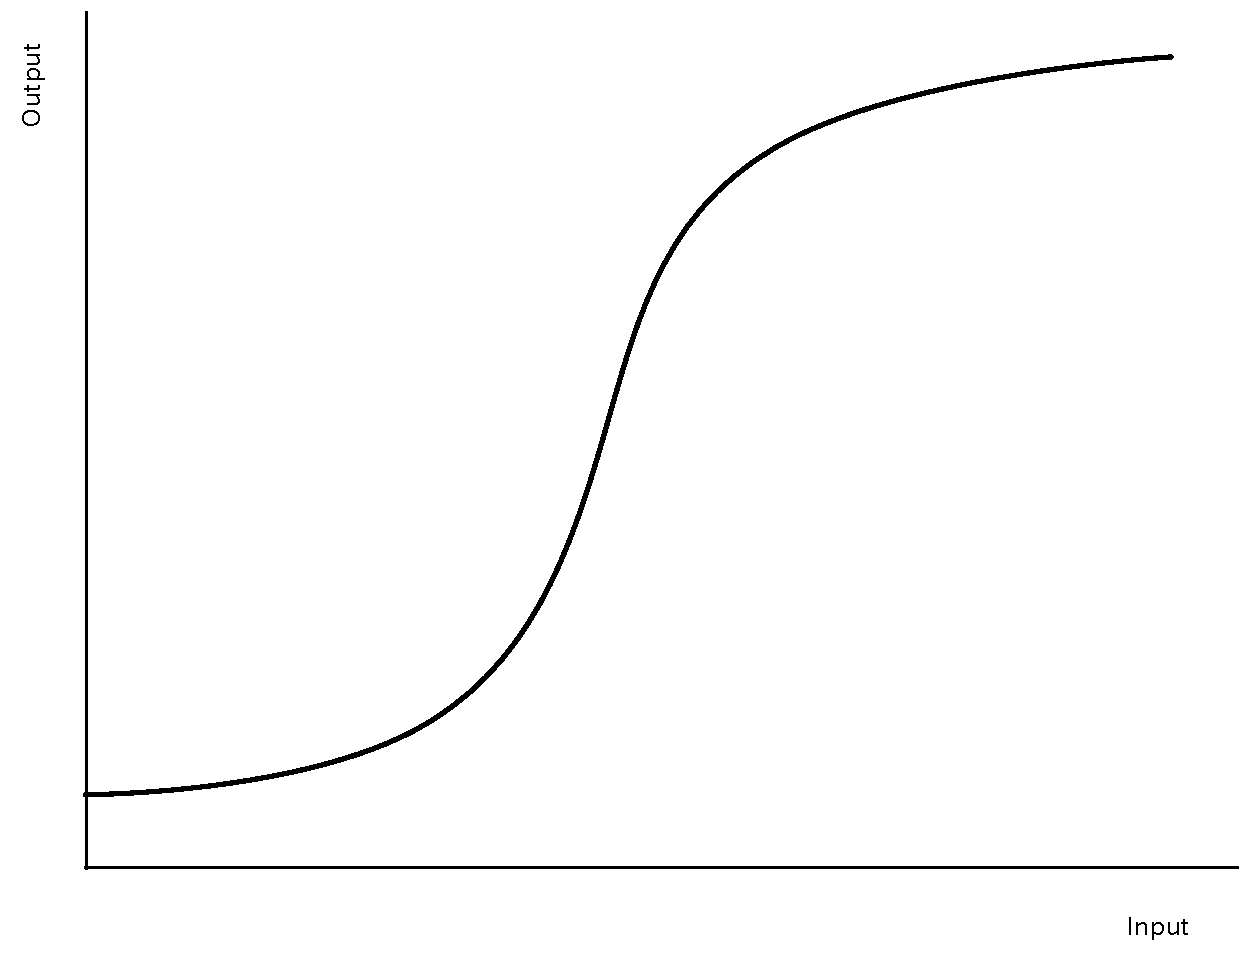
\includegraphics[scale=.35]{plot58.pdf}}
				\caption{Standard Production Function}
		\end{figure}
\end{frame}

\begin{frame}{The Costs of Production - Properties}
	\begin{enumerate}
		\item $MC$ still increases after some $Q$.
		\item $ATC$ still u-shaped.
		\item $MC$ crosses $ATC$ and $AVC$ at their minimum.
	\end{enumerate}
\end{frame}

\begin{frame}{The Costs of Production - The Long Run}
\begin{itemize}
	\item 	In the short run, a firm cannot get rid of its \dd{fixed costs} because they are \dd{sunk}. However, in the long run, these costs become \dd{variable}.
\end{itemize}
	\begin{figure}[H]
		\centering
		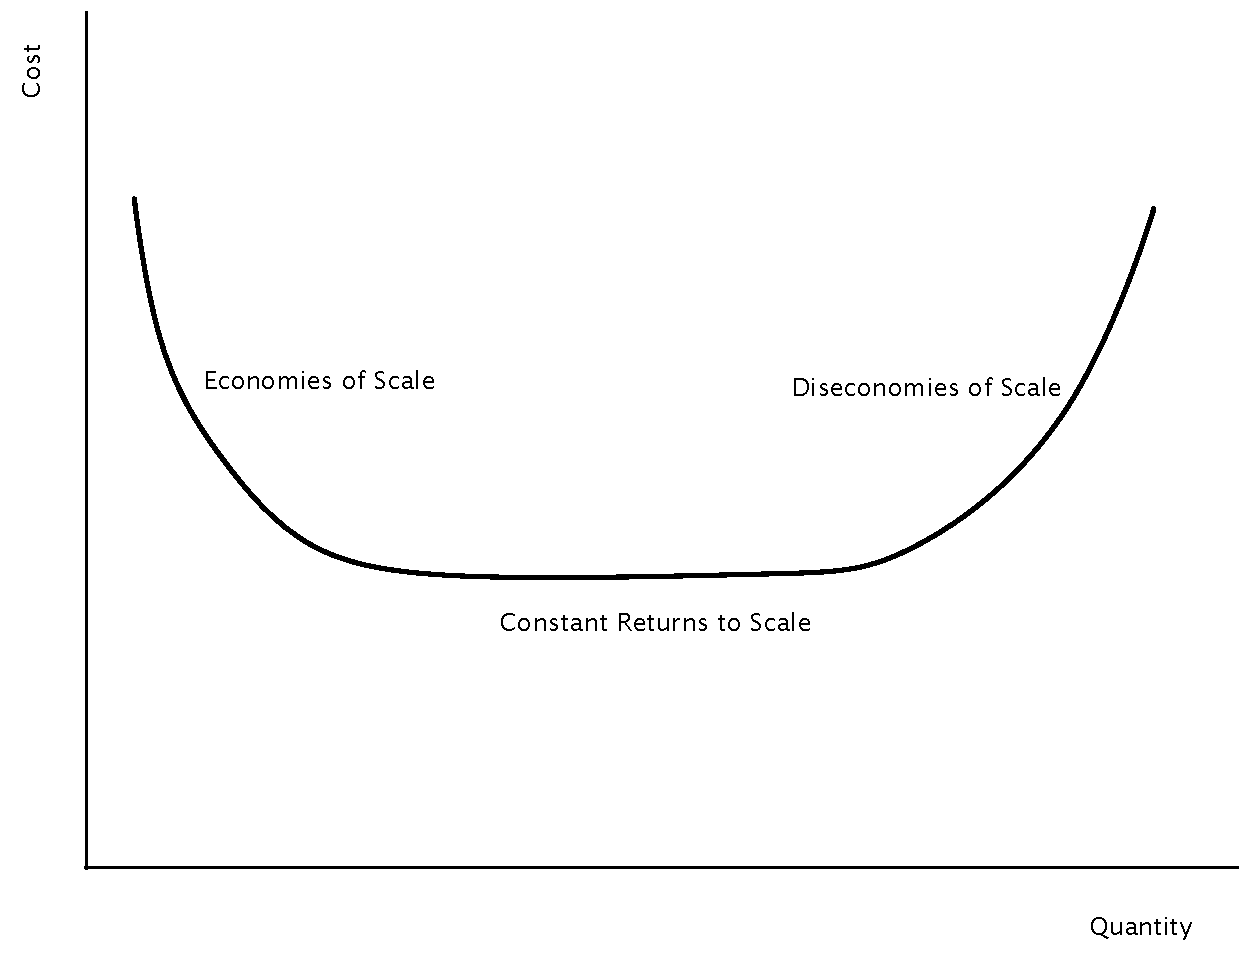
\includegraphics[scale=.3]{plot60.pdf}
		\caption{Long-Run ATC}
	\end{figure}
\end{frame}

\begin{frame}{The Costs of Production - The Long Run}
\begin{itemize}

		\item \defn{Economies of Scale:} Property whereby long-run $ATC$ decreases as $Q$ increases.
		\item \defn{Constant Returns to Scale:} Property whereby long-run $ATC$ remains constant as $Q$ increases.
		\item \defn{Diseconomies of Scale:}  Property whereby long-run $ATC$ decreases as $Q$ increases.
\end{itemize}
\end{frame}



\begin{frame}{Readings and Assignments}
\begin{itemize}
	\item Today: Mankiw Ch. 13
	\item Next time: Mankiw Ch. 14
	\item Problem Set 3, section 1
\end{itemize}
\end{frame}

\end{document}